%% Cambiare qui sotto con pdfLaTeX o LuaLaTeX a seconda del compilatore da usare

% !TEX TS-program = LuaLaTeX
% !TEX encoding = UTF-8 Unicode
% !BIB TS-program = biber

% Composizione in vari formati a seconda dell'opzione:
% a4paper, a5paper, b5paper, tablet, pad

%\documentclass[b5paper,11pt,ipertesto,oneside]{guidatematica}
%\documentclass[tablet,9pt,ipertesto,openany]{guidatematica}
\documentclass[b5paper,11pt,oneside]{guidatematica}
\ProvidesFile{bibliografia.tex}[2019/07/16 v.2.1.3 I software bibliografici e BibLaTeX]
\setotherlanguages{english,german}

\usepackage{array,longtable,tabularx}

%%% Questa riga mancava nella versione 1.4b e la compilazione non andava
%%% a buon fine con pdflatex.
\ifPDFTeX
   \usepackage{amsmath,amssymb}
\else
   \let\originaldots\dots
   \renewcommand\dots{\ifmmode\originaldots\else.\kern1pt.\kern1pt.\fi}
   \setmathfont{Latin Modern Math}
\fi
%%%

%\DeclareRobustCommand*{\Ars}{%
%  \textsf{\lower -.48ex\hbox{\rotatebox{-20}{A}}\kern -.3em{rs}}\hskip0pt%
%  \kern -.05em\TeX\hskip0pt\kern -.17em\lower -.357ex\hbox{nica}}


%\makeindex[options={-s guidatematica.ist},intoc]

%\hfuzz=1pt

\usepackage{xpatch}

\usepackage[autostyle,italian=guillemets]{csquotes}
\usepackage[backend=biber,%block=ragged,
	annotate=true,short,reflist,% reflist=autore-data
	giveninits=true,% solo iniziale del nome in bibliografia
		style=windycity,hyperref]{biblatex}
\DeclareFieldFormat{annotation}{\par{\small{#1}}}
\renewcommand{\mkbibnamefamily}[1]{\textsc{#1}}% cognome autori in maiuscoletto in bib
%\DeclareFieldFormat{url}{\newline{\url{#1}}}
\DeclareFieldFormat{note}{\textcolor{brown}{#1}}
\addbibresource{guida.bib}
\addbibresource{guida2.bib}
%\usepackage{indentfirst}

\lstdefinestyle{es}{frame=lines,%
	basicstyle={\ttfamily\small},%
	breaklines=true,%
	escapeinside={(*@}{@*)}}
\lstdefinestyle{cmd}{frame=lines,%
	basicstyle={\small},%
	language=[LaTeX]{TeX},%
	keywordstyle=\ttfamily,%
	commentstyle=\itshape,%
	breaklines=true,%
	mathescape=true,%
	escapeinside={(*@}{@*)}}
\usepackage[scale=2]{ccicons}
\usepackage{hologo}
\usepackage{titling}
%\usepackage{guit}
%\usepackage{sectsty}
%\allsectionsfont{\sffamily}

\usepackage{hyperref}
%\hypersetup{colorlinks=true,urlcolor=red,citecolor=cyan,breaklinks,bookmarksopen}

\DeclareSourcemap{
  \maps[datatype=bibtex, overwrite]{
    \map{
      \perdatasource{guida.bib}
      \step[fieldset=KEYWORDS, fieldvalue=latex, append]
    }
    \map{
      \perdatasource{guida2.bib}
      \step[fieldset=KEYWORDS, fieldvalue=others, append]
    }
  }
}

\newcommand{\eng}[1]{\textenglish{\emph{#1}}}

\begin{document}

\author{Filippo Vomiero}
\title{Utilizzare i software per la gestione della bibliografia con \LaTeX}
\GetFileInfo{\jobname.tex}
\date{Versione \fileversion\ del \filedate}
\licenza{\thetitle\\%
Filippo Vomiero, \the\year\vspace{\baselineskip}\\%
Opera distribuita con licenza \textsf{Creative Commons}\\\textsf{Attribution-ShareAlike 4.0 Internazionale}\bigskip\\%
\href{https://creativecommons.org/licenses/by-sa/4.0/deed.it}{\ccbysa}}

\maketitle

\chapter{Introduzione}
Questa guida affronta l'argomento della bibliografia in \LaTeX, o, più precisamente, di come scrivere una bibliografia con il pacchetto \pack{biblatex}, utilizzando dei software esterni per la gestione del database bibliografico. Esula dallo scopo (e da quello di una guida tematica) introdurre concetti e comandi di base, che verranno dati per scontati. Il neofita può trovare indicate alcune guide di base da cui iniziare nella bibliografia \LaTeX\ a pagina~\pageref{bib}, oppure nella sezione ``documentazione'' sul sito del \GuIT, assieme a molto altro materiale interessante.

Questo documento è, in primo luogo, frutto del mio lavoro come bibliotecario presso l'Università degli Studi di Padova. Il Sistema Bibliotecario di Ateneo ormai da molti anni offre a studenti e docenti dei corsi di formazione su alcuni software per la gestione della bibliografia, quelli che vengono chiamati \eng{reference manager} o \eng{bibliographic manager} in inglese. Mi è stato chiesto da dei colleghi se fosse possibile predisporre una breve guida che illustrasse l'integrazione tra questi software e \LaTeX; dopo alcuni esperimenti, ho scritto una prima versione che è stata pubblicata sul sito del nostro Sistema Bibliotecario.

Poiché non mi sentivo (e non mi sento tuttora) un grande esperto di \LaTeX, ho chiesto un parere a chi ne sa molto più di me, scrivendo un post sul forum del \GuIT. Mi ha risposto prontamente Claudio Beccari, il quale, oltre a fornirmi preziosi suggerimenti per migliorare il lavoro, mi ha anche indicato la strada per trasformare il mio lavoro in una nuova guida tematica. Quanto segue è frutto di una lunga revisione; il contenuto è stato ampliato includendo alcune nozioni di base di bibliografia, e si è rivisto il documento per sfruttare i comandi della classe \class{guidatematica}.

Invito chiunque leggerà e farà uso di questa guida a contribuire alla stessa, segnalandomi sia gli errori, sia i suggerimenti che verranno ritenuti più opportuni. Un lavoro collettivo è sicuramente migliore di uno individuale.

\chapter*{Ringraziamenti}
In primo luogo, voglio ringraziare le colleghe Elisa Rubino e Silvia Sartorelli: i loro consigli sono stati preziosi per rifinire la prima versione di questa guida. Un ringraziamento particolare a Claudio Beccari: ha sopportato le mie numerose email, rispondendo con pazienza a tutti i miei dubbi e quesiti, e mi ha aiutato a conoscere meglio alcuni dei meccanismi nascosti di \LaTeX. Ma, soprattutto, quando \emph{OldClaudio} ti risponde chiedendoti di scrivere una Guida Tematica per il \GuIT, sai di aver fatto un buon lavoro, e, per me, questo vale tanto quanto un assegno di Knuth.
\begin{flushright}
\begin{minipage}{0.6\textwidth}\centering
\textsc{Filippo Vomiero}\\
\texttt{filippo[dot]vomiero[at]unipd[dot]it}
\end{minipage}
\end{flushright}
\newpage
%{\hypersetup{linkcolor=cyan}
\tableofcontents*
%}
\clearpage

\mainmatter*

\chapter{La bibliografia in \LaTeX}
\label{intro}
In \LaTeX\ è possibile compilare una bibliografia in due modi:%
%\renewcommand{\descriptionlabel}[1]{\hspace*{\labelsep}\textsc{#1}}
\begin{description}
\item[manuale] È il metodo nativo di \LaTeX, che utilizza un ambiente apposito, chiamato \amb{thebibliography}. È relativamente facile da usare, ma ha anche molte limitazioni, e comporta una serie di operazioni che vanno eseguite manualmente di volta in volta:\footnote{L'argomento è trattato in molte guide di base, come \parencites[71--72]{lamport:latex}[123--125]{pantieri:arte}[178--179]{guit}.}
	\begin{compactitemize}
	\item l'ordinamento delle voci in bibliografia non è automatico;
	\item se si aggiorna o modifica un riferimento bibliografico, bisogna andare a modificare le bibliografie di tutti i documenti in cui esso appare;
	\item se si desidera cambiare lo stile dei riferimenti bibliografici, bisogna cambiare a mano \emph{tutte} le voci, una per una.
	\end{compactitemize}
\item[automatico] Per ovviare ai problemi del metodo manuale, è decisamente preferibile utilizzare un database esterno contenente i nostri riferimenti bibliografici (tipicamente un file \file{*.bib}), e poi utilizzare un pacchetto di stile che formatterà in modo automatico tutti i riferimenti bibliografici inseriti nel testo.
\end{description}
In questa guida vedremo come utilizzare il metodo automatico, a partire dal capitolo~\ref{auto}. Prima di proseguire, però, meglio dedicare un istante per chiarire alcuni termini che verranno usati con frequenza.

\section{Citazioni e riferimenti}
La lingua inglese ha dei termini abbastanza precisi per identificare i diversi elementi: con \eng{quotation} indica la trascrizione (o la parafrasi) di un testo a cui si vuol far riferimento, mentre \eng{citation} è l'indicazione degli elementi bibliografici necessari per identificare l'opera a cui si vuol fare riferimento. La norma sui riferimenti bibliografici, la norma ISO 690 \parencite{iso690}, distingue ulteriormente: \eng{citation} sono le indicazioni bibliografiche inserite nel testo (indipendentemente dalla forma o posizione; possono essere, quindi, tra parentesi o in nota a piè di pagina), mentre definisce \eng{reference} l'insieme di dati che che descrivono una risorsa (bibliografica), sufficientemente precisi per identificarla e localizzarla. \LaTeX\ segue la logica di questa norma: il comando \comando{\cite} (e gli altri comandi derivati, vedi \ref{comandi}), inserisce nel testo una indicazione bibliografica specificata in precedenza, e la bibliografia è una lista ordinata di queste indicazioni bibliografiche, i \eng{reference}.

La situazione in italiano è un po' diversa.%
\footnote{Esiste una versione italiana della norma ISO 690, pubblicata dall'UNI (UNI ISO 690:2007, non aggiornata; la più recente UNI ISO 690:2014, attualmente in vigore, mantiene il testo inglese) che traduce \eng{citation} con `citazione', e \eng{reference} con `riferimento'. Tuttavia, vedendo che nel capitolo~3, ``Termini e definizioni'', viene definito `editore' la ``persona o organizzazione responsabile della produzione e della distribuzione di un documento'' \parencite[3]{uni690}, per poi utilizzare il medesimo termine nel capitolo~7 al posto di `curatore' per tradurre \eng{editor}, viene da chiedersi se il gruppo di lavoro non abbia tradotto con troppa leggerezza cadendo nel classico tranello dei \eng{false friends}. Pertanto, ho preferito non considerare vincolante la scelta terminologica operata dalla norma.}
Secondo \emph{Il Vocabolario Treccani}, il verbo \emph{citare} ha due significati: il primo riguarda la chiamata in giudizio, con varie sfumature; poco rilevante in questa sede. Il secondo significato viene invece definito così: ``Allegare, riportare parole di persone o di testi autorevoli, ricordare fatti o episodî a conferma di quanto di sostiene; riferire passi di opere, sia per esemplificazione, sia anche per semplice diletto estetico'' \parencite[800]{treccani}.
Si può, quindi, tradurre fedelmente \eng{to quote} con questo verbo, e, di conseguenza, \eng{quotation} con ``citazione''. La situazione si complica però quando si prova a tradurre \eng{citation}, che ha anche lo svantaggio di essere foneticamente molto simile alla parola appena utilizzata. Sempre \emph{Il Vocabolario Treccani}, alla voce \emph{citazione}, indica, come ultimo significato (2b), il suo uso per riportare le informazioni bibliografiche: ``Indicazione del titolo, volume, pagina di un'opera [\ldots] alla quale si rimanda per stabilire rapporti con quanto si scrive o si dice, oppure per dare autorità a quanto si afferma, per precisare le fonti alle quali si attinge'' \parencite[800]{treccani}.
Alfredo Serrai \parencite[31]{serrai} per differenziare i significati usa due circonlocuzioni: la \emph{citazione testuale} ``è la ripresa e l'inserimento di un testo pubblicato, o di una sua parte, in un altro testo'', mentre la \emph{citazione bibliografica} ``di natura simbolico--linguistica, è il riferimento compendiato ad un'opera in funzione di indice della stessa''.

Personalmente, preferisco evitare l'uso di uno stesso termine con due significati diversi nel medesimo documento, perché è facile generare fraintendimenti o, quantomeno, confusione. Una soluzione può essere quella di utilizzare delle specificazioni, come, ad esempio, quelle suggerite da Serrai; tuttavia, in un documento come questo, dove può essere molto frequente il ricorso a elementi di natura bibliografica, trovo non molto pratiche le circonlocuzioni: esse rendono il discorso poco agevole, appesantendo le frasi. Ho quindi scelto dei termini che potessero essere utilizzati in maniera univoca, indicando sempre e solo lo stesso elemento, e ho cercato di utilizzarli con coerenza fino alla fine. In questa guida ``citazione'' indica il testo riportato a cui si fa riferimento (l'inglese \eng{quotation}), mentre  ``riferimento (bibliografico)'' è usato per tutte le indicazioni bibliografiche, siano esse inserite nel testo, o in bibliografia, traducendo sia \eng{citation} che \eng{reference} secondo la specificazione della norma ISO 690. Mi perdoni l'utilizzatore abituale di \LaTeX\ che probabilmente avrà trovato in molte guide un'espressione simile a ``inserire una citazione nel testo con il comando \cs{cite}''; in questa guida viene sempre detto che \cs{cite} inserisce un \emph{riferimento (bibliografico)} (\ref{comandi}): con questo paragrafo spero di aver chiarito la questione.

\section{Lo stile dei riferimenti bibliografici}
Quando si affronta l'argomento della bibliografia e dei riferimenti bibliografici da inserire in un testo, si deve necessariamente trattare anche la questione dello \emph{stile} che tali elementi devono avere. I manuali di stile sono dei testi che stabiliscono una serie di regole e buone pratiche di scrittura, che possono riguardare la grammatica, la punteggiatura, l'ortografia, le abbreviazioni, e, per l'appunto, i riferimenti bibliografici. In senso stretto si parla di \emph{stile citazionale} quando ci si vuol riferire specificamente a questo ambito. Lo stile citazionale è quindi quell'insieme di regole che definisce, in primo luogo, quali elementi devono comparire nel testo e in che ordine (uno stile del tipo ``autore--data'', ad esempio, inserirà il riferimento tra parentesi, ed esso sarà composto solamente dal cognome dell'autore e dall'anno di pubblicazione), e definisce anche con quali caratterizzazioni tipografiche un elemento del riferimento può essere evidenziato (ad esempio, distinguendo il titolo di un articolo o di una parte di libro tra virgolette, e il titolo del contenitore, rivista o libro, in corsivo).%
\footnote{Questa spiegazione può diventare più chiara guardando come è scritta la voce ``La citazione bibliografica'' \parencite{serrai}, a pagina~\pageref{bib2}.}

In \LaTeX\ il compito di conformare riferimenti e bibliografia a uno stile specifico è svolto da dei pacchetti di gestione automatica della bibliografia.

\chapter{La gestione automatica della bibliografia in \LaTeX}\label{auto}
La gestione automatica è stata implementata in \LaTeX\ attraverso un programma esterno chiamato \prog{bibtex}. Il programma originariamente supporta solo la codifica ASCII, in un secondo momento è stata prodotta una seconda versione che supporta i caratteri a 8-bit, chiamata \prog{bibtex8} e anche una con supporto a UTF-8, chiamata \prog{bibtexu}, mantenendone inalterate le capacità. Nel 2006 è stato creato un secondo programma, \prog{biber}, che, assieme al pacchetto \pack{biblatex}, offre più flessibilità e funzionalità.%
\footnote{L'impostazione generale dei pacchetti basati su \prog{bibtex} è pensata per la lingua inglese, con delle differenze significative non proprio adatte per i lavori in lingua italiana; inoltre, il linguaggio di markup usato dagli stili citazionali che si appoggiano ad esso non è quello standard di \LaTeX, per cui le modifiche a uno di essi, anche di modesta entità, risultano piuttosto complesse.}

\section{Programmi e pacchetti}
Prima di continuare, è bene fare un po' di chiarezza su alcuni termini che verranno usati frequentemente.%
\footnote{Un eccellente approfondimento è reperibile al seguente indirizzo:\\
\href{https://tex.stackexchange.com/questions/25701/bibtex-vs-biber-and-biblatex-vs-natbib}{\texttt{https://tex.stackexchange.com/questions/25701/bibtex-vs-biber-and-biblatex\discretionary{}{-}{-}vs-natbib}} 
Visitato il 21 maggio 2019.}
In senso stretto \prog{bibtex} è il nome del programma esterno che gestisce le informazioni bibliografiche contenute in un database (un file \file{*.bib}) e le integra in un documento \LaTeX\ (\ref{printbib}), sfruttando i comandi messi a disposizione da un particolare pacchetto, potendo così stabilire lo stile della bibliografia. Tuttavia, spesso il termine è stato usato per indicare elementi differenti, generando un po' di confusione. I software di gestione bibliografica, ad esempio, chiamano ``file bibtex'' il file \file{*.bib} contenente il database bibliografico. Oppure ancora, è facile trovare l'indicazione "gestire la bibliografia con \hologo{BibTeX}" la quale in realtà riassume più operazioni: non compilare la bibliografia con il metodo manuale descritto nella sezione precedente, bensì salvare i riferimenti in un file \file{*.bib} e utilizzare un pacchetto che permetta, sfruttando il programma \prog{bibtex}, di inserire e formattare automaticamente i riferimenti bibliografici e la bibliografia.

Una classificazione precisa deve quindi distinguere:
\begin{description}
\item[programmi]\prog{bibtex} e \prog{biber} sono due programmi esterni; la loro interazione con \LaTeX\ è illustrata nella sezione~\ref{printbib}.
\item[pacchetti]\pack{natbib} e \pack{biblatex} sono due pacchetti che permettono di formattare i riferimenti e la bibliografia. \pack{natbib} funziona solo con \prog{bibtex} e storicamente è stato il pacchetto più utilizzato. \pack{biblatex} invece è sviluppato assieme a \prog{biber} ed è con esso che funziona al meglio, ma, al momento, mantiene la retro-compatibilità con \prog{bibtex}, ed è possibile utilizzarlo con questo programma indicandolo nelle opzioni.
\end{description}

Per evitare confusione, quindi, quando nel testo i termini compariranno con la grafia appena utilizzata, il riferimento sarà specifico: \prog{bibtex} indica il programma e \pack{biblatex} il pacchetto. Tuttavia, capiterà spesso di dover fare riferimento ai due ambienti di lavoro in senso più generale, così come ormai è entrato nel linguaggio comune (gli stessi software di gestione bibliografica presi in analisi nel capitolo~\ref{database} utilizzano i termini in questo senso). In queste occasioni, si utilizzerà la scrittura logografica \hologo{BibTeX} e Bib\LaTeX, indicando in tal modo l'intero ecosistema programma più pacchetto: \prog{bibtex}+\pack{natbib} nel primo caso, \prog{biber}+\pack{biblatex} nel secondo.
 
\section{Pacchetti per la gestione della bibliografia}
Qui di seguito sono elencati alcuni pacchetti che permettono di gestire automaticamente la bibliografia.
%\renewcommand{\descriptionlabel}[1]{\hspace*{\labelsep}\textbf{\pack{#1}}}
\begin{plaindescription}[before={\renewcommand\makelabel[1]{\pack{##1}}}]
\item[\href{https://ctan.org/pkg/natbib}{natbib}] È uno dei pacchetti  di stile per \prog{bibtex} più famosi e utilizzati, ha il grosso vantaggio che negli anni sono stati creati degli stili per i principali  editori scientifici. Tuttavia non è più aggiornato e quindi, in prospettiva futura, sarebbe meglio migrare verso altri pacchetti. Al momento rimane, comunque, molto valido.
\item[\href{https://ctan.org/pkg/jurabib}{jurabib}] Altro pacchetto di stile per \prog{bibtex}, nato per far fronte alle complessità dei riferimenti bibliografici in ambito giuridico, ma che è ampiamente adattabile. Anche questo, tuttavia, non è più aggiornato dal suo autore.
\item[\href{https://ctan.org/pkg/biblatex}{biblatex}] Pacchetto costantemente aggiornato ed estremamente versatile, sviluppato congiuntamente al programma di backend \prog{biber}, che amplia di molto le funzionalità offerte da \prog{bibtex} e dai pacchetti basati su di esso, pur mantenendo la retrocompatibilità. È provvisto di cinque stili citazionali predefiniti, ma su \href{https://ctan.org/}{CTAN} \textenglish{(Comprehensive \TeX\ Archive Network)} se ne possono reperire molti altri, che coprono sia alcuni dei principali manuali di stile, sia stili specifici di editori (vedi la sezione~\ref{stili} per una lista sintetica). Questa guida si concentra esclusivamente su questo pacchetto.%
\footnote{Cercando su CTAN il \emph{topic} ``biblatex'' si ottiene una lista di tutti gli stili attualmente disponibili.\\%
\url{https://ctan.org/topic/biblatex}}
\end{plaindescription}

\chapter{Il database bibliografico}\label{database}
Come anticipato nel capitolo \ref{intro}, una bibliografia gestita automaticamente utilizza un database esterno, interpretato da un programma, (\prog{bibtex} o \prog{biber}), che ne ricava i riferimenti bibliografici, i quali vengono inseriti in un documento secondo uno stile citazionale gestito da un pacchetto come \pack{biblatex}, che a sua volta può servirsi di pacchetti aggiuntivi per impostare lo stile.%
\footnote{Nella compilazione di questa guida è stato utilizzato il pacchetto \href{https://ctan.org/pkg/windycity}{\pack{windycity}} per formattare riferimenti bibliografici e bibliografia finale secondo il \emph{Chicago Manual of Style}, a cui ho aggiunto alcune modifiche manuali per renderlo più vicino allo stile delle altre guide tematiche.}

\hologo{BibTeX} prevede i database in un file di testo, da non compilare, con estensione \file{*.bib}, e questo rimane il formato più comune.  Bib\LaTeX\ ha una struttura di dati leggermente diversa da \hologo{BibTeX}, per cui può essere necessario modificare manualmente il file passando da uno all'altro, come indicato nella guida del pacchetto al capitolo~2.3, ``Usage notes'' \parencite[123--125]{biblatex}.
Alcuni software di gestione della bibliografia, come \prog{Zotero} o \prog{Jabref} supportano anche l'esportazione di un database bibliografico in formato Bib\LaTeX.

Nelle sezioni successive indicherò l'insieme dei dati che compongono il riferimento bibliografico con l'espressione ``record (bibliografico)''. In informatica indica genericamente un oggetto di un database, che è a sua volta un insieme di campi (o elementi), composto da un identificatore univoco e un dato. In biblioteconomia il record bibliografico viene utilizzato esattamente allo stesso modo, con la sola specificazione che i dati sono informazioni bibliografiche. Appare evidente guardando la struttura di un database \file{*.bib}.

\section{La sintassi di un file \texttt{*.bib}}\label{syntax}
La bibliografia, intesa come disciplina, individua alcuni elementi fondamentali per identificare un documento a cui si fa riferimento.
\begin{description}
\item[responsabilità] Il responsabile dei contenuti generalmente è l'autore, ma in sua mancanza può esserci il curatore, oppure in altri casi un \emph{autore collettivo} come nel caso di enti o associazioni
\item[data] Informazione molto importante per contestualizzare un'opera. Data e indicazione di responsabilità sono i due elementi generalmente richiamati quando si inserisce un riferimento bibliografico direttamente nel testo senza ricorrere a note
\item[titolo] Normalmente riportato per intero, serve a individuare il documento, e, di norma, ci dà un'idea del suo contenuto
\item[contenitore] Se esiste, serve a localizzare un documento all'interno di un altro: il caso più comune è quello di un articolo pubblicato in una rivista
\end{description}
A questi si sommano altri elementi che possono facilitare il reperimento di un documento, come, ad esempio, l'indicazione di edizione, il luogo di pubblicazione e l'editore o il numero di pagine. L'appendice B della norma ISO 690, illustra quali sono gli elementi obbligatori e quali quelli facoltativi, a seconda della tipologia di materiale \parencite[28--32]{iso690}.

In modo analogo anche il \eng{data model} di Bib\LaTeX, mutuato da quello di \hologo{BibTeX}, prevede dei campi obbligatori e altri facoltativi, a seconda della tipologia di documento \parencite[6--44]{biblatex}.
Per capire come compilare manualmente un file \file{*.bib}, vediamo un esempio:
\begin{lstlisting}[style=es]
@book{lamport:latex,
	location = {Reading, Mass. [etc.]},
	title = {LaTeX: a document preparation system. User's guide and reference manual},
	edition = {2},
	isbn = {0-201-52983-1},
	pagetotal = {{XVI}, 272 p., [1] p. di tav. ripieg.},
	publisher = {Addison-Wesley},
	author = {Lamport, Leslie},
	date = {1994}
}
\end{lstlisting}
La prima riga contiene due informazioni: la \emph{tipologia di documento}, inserita dopo il carattere \texttt{@}, e l'\emph{etichetta} (in molte guide chiamata \textit{chiave}), un nome arbitrario assegnato al record per identificarlo, nell'esempio \texttt{lamport:latex}. La tipologia di documento determina quali saranno i campi obbligatori e quelli facoltativi. Tra le tipologie più comuni, ad esempio, \texttt{book}, che indica le monografie, prevede come obbligatori i campi \texttt{author}, \texttt{title} e \texttt{year/date}; \texttt{article}, che indica gli articoli,  richiede \texttt{author}, \texttt{title}, \texttt{year/date} e \texttt{journaltitle}; \texttt{online}, che indica le risorse online (prevalentemente pagine web), richiede i seguenti campi: \texttt{author/editor}, \texttt{title}, \texttt{year/date} e \texttt{url}. 


Come si può vedere nell'esempio, ciascun campo è separato da virgole; la sintassi prevede questa formulazione:\\[1ex]
%\begin{lstlisting}[style=cmd]
%(*@$\langle$\textit{nome del campo}$\rangle$@*) = {(*@$\langle$\textit{contenuto del campo}$\rangle$@*)}
%\end{lstlisting}
\begin{tabularx}{\linewidth}{@{}X@{}}
\toprule
\meta{nome del campo} = \Marg{\meta{contenuto del campo}}\\
\bottomrule
\end{tabularx}\\[1ex]
L'intero record, dopo l'indicazione della tipologia, è racchiuso tra parentesi graffe.

Per quanto concerne il campo \texttt{edition}, \pack{biblatex} prevede che esso sia un numero intero, così verrà sfruttato il pacchetto \pack{babel} per inserire nel testo l'indicazione di edizione corretta secondo la lingua in uso, trasformando il numero in ordinale (che non va quindi inserito nel campo). Nel caso di indicazioni testuali di edizione, come, ad esempio, ``nuova edizione riveduta e corretta'', essa va inserita integralmente nel campo, così come desideriamo appaia nel testo: in questo caso, infatti, \pack{biblatex} riporta alla lettera il contenuto del campo senza applicare modifiche.

Il campo \texttt{date} indica la data di pubblicazione. Per motivi di compatibilità con \hologo{BibTeX} viene mantenuto anche il campo \texttt{year}, ma la guida del pacchetto \pack{biblatex} consiglia di usare il campo \texttt{date}, che ha molte più funzioni. La data va inserita nel formato $\langle$\textit{anno--mese--giorno}$\rangle$, ad esempio \{\texttt{2018-12-31}\}. Il trattino separa sempre le scansioni temporali: l'anno dal mese dal giorno. È possibile inserire anche degli intervalli di date (sia chiusi che aperti), utilizzando la barra obliqua (o \emph{slash} in inglese), ad esempio: \{\texttt{1997/1998}\} viene riprodotto ``1997--1998'', mentre un intervallo aperto \{\texttt{1981/}\} diventa ``1981--''. L'argomento è trattato nel capitolo~2.3.8, ``Date and time specifications'', della guida al pacchetto \pack{biblatex} \parencite[37--39]{biblatex}.

È sempre preferibile utilizzare la tipologia più aderente al tipo di materiale, anche quando una risorsa si presenta in versione elettronica, come molte riviste pubblicate solo digitalmente. In questi casi, va usato \texttt{@article} inserendo nel campo \texttt{url}, che è supportato da tutte le tipologie, il link all'articolo sul sito dell'editore. Lo stesso discorso si applica per gli ebook. Quando vengono utilizzati materiali \emph{elettronici}, cioè risorse di cui è stata consultata una versione online, va utilizzato il campo \texttt{urldate} che indica la data dell'ultima visita alla risorsa: il campo è facoltativo per Bib\LaTeX, ma la norma ISO 690 lo indica come obbligatorio, ed è raccomandato dai manuali di bibliografia.

\section{Creare un file \texttt{*.bib}}
Molti \eng{shell editor} comprendono funzioni per la scrittura facilitata di un file \file{*.bib}, e con essi è possibile compilarlo manualmente senza troppe difficoltà. In questa operazione, tuttavia, i software di gestione bibliografica possono essere di grande aiuto: tramite di essi, infatti, oltre a poter gestire e organizzare i nostri riferimenti bibliografici, è possibile esportare facilmente i riferimenti utilizzati nel nostro lavoro.

Esula dallo scopo di questa guida elencare i diversi software, mettendone in evidenza caratteristiche comuni e differenze, per cui ci si limiterà a portare gli esempi di \prog{Zotero} e di \prog{Mendeley}, che sono i due software a cui il Sistema bibliotecario dell'Università degli studi di Padova fornisce supporto, a cui ho aggiunto il software \prog{Jabref}, che è progettato specificatamente per lavorare in \LaTeX\ e facilita di molto le operazioni di compilazione della bibliografia.

\subsection{Zotero}
Per creare un file \file{*.bib} con \prog{Zotero}, si consiglia di inserire tutti i riferimenti richiesti in un'unica cartella, quindi dall'applicazione desktop di \prog{Zotero}, fare click con il tasto destro sulla cartella, e selezionare la voce \verb!Esporta collezione!, a questo punto si apre una finestra che chiede di selezionare alcune impostazioni: come formato selezionare \texttt{biblatex}; secondo necessità è possibile esportare anche le note, che poi compariranno come commenti in bibliografia, come fatto in questa guida (\ref{bibnote}); infine come codifica caratteri selezionare \verb!UTF-8! (dovrebbe essere l'impostazione predefinita): questo permette di non dover modificare i vari caratteri speciali che compaiono nei riferimenti, visto che Bib\LaTeX, a differenza di \hologo{BibTeX} supporta tale codifica. Il nome predefinito del file che verrà creato è quello della cartella, consigliamo di dare lo stesso nome del file \file{*.tex} su cui vogliamo lavorare.

L'architettura aperta di \prog{Zotero} permette l'integrazione con svariate estensioni: tramite di esse vengono introdotte migliorie e nuove funzioni, ed è possibile l'integrazione con altri programmi.%
\footnote{Cfr. \url{https://www.zotero.org/support/plugins} per una lista delle estensioni disponibili.}
All'utilizzatore di \LaTeX\ interesserà sicuramente l'estensione ``Better BibTeX'' che rende più facile e precisa l'esportazione di un database bibliografico per \hologo{BibTeX} o Bib\LaTeX. Per una descrizione del progetto si veda: \url{https://github.com/retorquere/zotero-better-bibtex} (Visitato il 27 giugno 2019).

\subsection{Mendeley}
Per creare un file \file{*.bib} con \prog{Mendeley}, si consiglia di inserire tutti i riferimenti richiesti in un'unica cartella, quindi dall'applicazione desktop di \prog{Mendeley}, entrare nella cartella e selezionare tutti i riferimenti, fare click con il tasto destro e selezionare la voce \verb!Export!. Il nome predefinito del file è \file{My Collection.bib}, si consiglia di utilizzare lo stesso nome del file \file{*.tex} su cui vogliamo lavorare. Come formato del file selezionare \texttt{BibTeX} (\file{*.bib}).

\subsection{Jabref}
Generalmente, un software di gestione della bibliografia utilizza un proprio database interno per memorizzare le informazioni relative ai record bibliografici di nostro interesse, ed è in grado di recuperare tali informazioni per fornirle secondo un formato specifico da noi selezionato: questa operazione viene chiamata solitamente \emph{esportazione}. Il grande vantaggio di \prog{Jabref} sugli altri software è che utilizza, come database interno dove salvare le informazioni, un file \file{*.bib} con il \eng{data model} di \hologo{BibTeX} o Bib\LaTeX, a seconda della scelta operata dall'utente. Questa caratteristica permette di non dover subire ``traduzioni'' di codici e linguaggi, bensì di lavorare direttamente nei campi previsti da Bib\LaTeX: il software ci segnalerà, a seconda della tipologia di documento, quali sono i campi obbligatori, e ci guiderà nella compilazione degli stessi. Inoltre è multi--piattaforma, e si integra con molti dei principali \eng{shell editor}. L'unico aspetto negativo, se confrontato con gli altri software, è che non possiede uno spazio di archiviazione in \eng{cloud} dove sincronizzare i nostri dati, così da poterlo utilizzare da più postazioni; per l'utilizzatore \LaTeX\ tuttavia, non è un problema insormontabile, basta tenere sempre assieme il file \file{*.tex} con quello \file{*.bib}, che sono solitamente file di piccole dimensioni e facilmente copiabili o inviabili via email.

\section{Controllare il file \texttt{*.bib}}
Dopo aver creato il database, è importante effettuare una revisione dei dati inseriti, sia per evitare errori in fase di compilazione con \LaTeX, sia per migliorare la resa tipografica dei riferimenti bibliografici. Questa fase di controllo è particolarmente importante se il file è stato creato utilizzando un software, ma verranno trattati alcuni aspetti che è bene conoscere anche nel caso di una compilazione manuale.

Partiamo con un esempio, creato con \prog{Zotero}:
\begin{lstlisting}[style=es]
@book{lehman_biblatex_2018,
	edition = {3.12},
	title = {The {bibLaTeX} Package},
	url = {https://ctan.org/pkg/biblatex},
	pagetotal = {322},
	author = {Lehman, Philipp and Kime, Philip and
	Wemheuer, Moritz},
	urldate = {2019-03-26},
	date = {2018-10-30},
	langid = {english},
	annotation = {Documentazione a corredo del pacchetto
	    {bibLaTeX}.}
}
\end{lstlisting}
Nella prima riga, dopo l'indicazione della tipologia di documento, è visibile l'etichetta generata automaticamente dal software (in inglese \eng{citekey}), \verb!lehman_biblatex_2018!: sarà con essa che il riferimento bibliografico verrà inserito nel testo tramite il comando \comando{\cite}, come descritto nella sezione~\ref{comandi}. Questa funzione dimostra tutta la sua utilità man mano che i riferimenti utilizzati si accumulano e diventano via via più numerosi. Quando i riferimenti sono pochi, è possibile rinominare le etichette in qualcosa di facile da memorizzare: una prassi comune è la sintassi \textit{$\langle$cognome$\rangle$:$\langle$parola significativa del titolo$\rangle$}, ad esempio \texttt{lehman:biblatex}, oppure la forma \textit{$\langle$cognome$\rangle\langle$anno$\rangle$}, che è anche utilizzata da \prog{jabref}: l'esempio di prima diventa \texttt{lehman2018}. È necessario che ciascuna etichetta sia univoca, altrimenti la compilazione si interromperà segnalando l'errore nel file di log: tutti i software qui menzionati svolgono un eccellente lavoro nell'evitare duplicati, ed è un ulteriore buon motivo per delegare a loro il compito di assegnare le etichette.

Di frequente sono necessarie alcune modifiche per ripulire i campi dai caratteri speciali utilizzati dai database da cui sono stati importati, o anche semplicemente per migliorare la resa tipografica dei riferimenti. Vediamo un esempio: il campo titolo è esportato da catalogo come \verb*!<<The >>LaTeX Companion!. In questo caso vanno eliminate le doppie parentesi uncinate che delimitano l'articolo.
Questo tipo di modifica, assieme all'inserimento delle note (\ref{bibnote}), si può fare nel file \file{*.bib}, ma consiglio di farlo direttamente all'interno del software di gestione bibliografica, così otterremo dei riferimenti puliti e pronti per essere utilizzati ripetutamente. Una modifica che invece è preferibile fare nel file \file{*.bib} è l'inserimento del comando \comando{\LaTeX} così da visualizzare correttamente il logo \LaTeX\ anche nei riferimenti e in bibliografia.\footnote{Ho rilevato, infatti, che i software proteggono il carattere speciale \textbackslash\ (\eng{backslash}), inserendo al suo posto il comando \cs{textbackslash} per visualizzare il segno corrispondente: il risultato è che in bibliografia compare il nome del comando che si voleva utilizzare, e non il logo.}

Un errore frequente che appare al momento della compilazione è dovuto all'uso, nel database bibliografico, di caratteri speciali riservati a funzioni specifiche di \LaTeX, come, ad esempio, il carattere ``\&'', che può comparire nel campo degli autori o del titolo: in \LaTeX\ è un cosiddetto \emph{carattere speciale}, il cui uso è riservato per separare le celle di una tabella. Per poter essere utilizzato all'interno del testo, va scritto con il suo comando apposito \comando{\&}. 

Altri errori riguardano per lo più i campi \texttt{autore} e \texttt{titolo}; nel primo caso se l'autore è un nome collettivo, come \textenglish{``Institute of Electrical Engineers''}, \hologo{BibTeX} potrebbe interpretare che \textenglish{``Institute''} è il nome proprio dell'autore, e \textenglish{``of Electrical Engineers''} il cognome. Per correggere questo comportamento, è sufficiente inserire tra virgolette il campo autore, o tra doppie graffe (solo in Bib\LaTeX). La stessa soluzione è valida anche quando un acronimo viene restituito solo con l'iniziale maiuscola e le altre lettere in minuscolo.

Tutti questi problemi dovrebbero essere gestiti in fase di esportazione dal software di gestione delle bibliografie, ma è sempre meglio controllare.%
\footnote{Dalle prove eseguite durante la compilazione di questa guida ho notato che i programmi con il supporto nativo a Bib\LaTeX\ come \prog{Zotero} (specialmente assieme all'estensione ``Better BibTeX'') o \prog{Jabref} risolvono la maggior parte di questi problemi, mentre è necessario un controllo per i software che esportano in formato \hologo{BibTeX}.}

\chapter{\textsc{Bib}\LaTeX}
Una volta terminate le operazioni sul file con il database bibliografico, si può procedere all'inserimento dei riferimenti bibliografici nel documento. Innanzitutto, va caricato il pacchetto \pack{biblatex}, inserendo queste righe nel preambolo:\\[1ex]
%\begin{lstlisting}[style=cmd]
%\usepackage[backend=biber,style=(*@$\langle$\textit{nome dello stile}$\rangle$@*)]{biblatex}
%\(*@\texttt{addbibresource}@*){(*@$\langle$\textit{nome file}$\rangle$@*).bib}
%\end{lstlisting}
%
\begin{tabularx}{\linewidth}{@{}X@{}}
\toprule
\cs{usepackage}\Oarg{backend=biber, style=\meta{nome dello stile}}\Marg{biblatex}\\
\cs{addbibresource}\Marg{\meta{nome file}.bib}\\
\bottomrule
\end{tabularx}\\[1ex]
La prima opzione specifica quale programma esterno usare, \prog{biber} è l'opzione di default, consigliata anche nella guida del pacchetto \parencite[45]{biblatex}, anche se è mantenuto il supporto a \prog{bibtex}, nelle due versioni \prog{bibtex} e \prog{bibtex8}, mentre è abbandonato il supporto a \prog{bibtexu}. L'opzione \texttt{style} va compilata con il nome dello \emph{stile citazionale} che si vuole adottare. \pack{biblatex} prevede cinque stili predefiniti (con alcune varianti), indicati nel capitolo~3.3 della guida \parencite[68--73]{biblatex}:
%\renewcommand{\plaindescriptionlabel}[1]{\hspace*{\labelsep}\textbf{\texttt{#1}}}
\begin{description}%[before={\renewcommand\makelabel[1]{\bfseries{\ttfamily{##1}}}}]
\item[numeric]I riferimenti appaiono solo con un etichetta numerica (1).
\item[alphabetic]Stile simile al precedente, ma l'etichetta è composta dalle prime lettere del cognome dell'autore e le ultime due cifre dell'anno di pubblicazione [Lam94].
\item[authoryear]Il riferimento è costituito dal cognome dell'autore e dall'anno di pubblicazione (Lamport, 1994).
\item[authortile]Il riferimento riporta il cognome dell'autore e il titolo, senza parentesi: Lamport, \LaTeX: a document preparation system.
\item[verbose]Il riferimento appare per intero, solitamente inserito in nota a piè di pagina.
\end{description}
Per \pack{biblatex} ciascuno stile è in realtà doppio: uno che gestisce i riferimenti bibliografici nel testo (salvato in un file \file{*.cbx}) e uno che gestisce la bibliografia (file \file{*.bbx}). Ovviamente i due devono coincidere, altrimenti diverrebbe difficile decifrare la bibliografia: è evidente con lo stile \texttt{numeric}, dove la bibliografia deve essere ordinata secondo l'ordine di apparizione dei riferimenti nel testo, e riportare le etichette numeriche di ciascun riferimento.

\section{Stili citazionali e pacchetti}\label{stili}
Oltre agli stili interni, è possibile caricare uno stile esterno, semplicemente dichiarando il nome del pacchetto nelle opzioni di \pack{biblatex}, come se fosse uno stile interno (l'unica differenza è che il pacchetto desiderato deve essere stato installato precedentemente). Qui di seguito si elencano alcuni degli stili disponibili, ma si rimanda nuovamente al \emph{topic} ``biblatex'' su \href{https://ctan.org/topic/biblatex}{CTAN} per una lista esaustiva.
%\renewcommand{\descriptionlabel}[1]{\hspace*{\labelsep}\textbf{\pack{#1}}}
\begin{description}[before={\renewcommand\makelabel[1]{\pack{##1}}}]
\item[\href{https://ctan.org/pkg/biblatex-apa}{biblatex-apa}]Stile che rispecchia fedelmente le indicazioni del manuale APA \textenglish{(American Psycological Association)}, 6\textsuperscript{a} edizione.
\item[\href{https://ctan.org/pkg/biblatex-chem}{biblatex-chem}]Pacchetto che racchiude più stili, utili per la chimica:%
\begin{compactitemize}
\item stile delle riviste ACS;
\item stile per le riviste della RSC che usano lo stile di \eng{Chem. Commun.};
\item stile per \textgerman{\emph{Angewandte Chem}}.
\end{compactitemize}
\item[\href{https://ctan.org/pkg/biblatex-ieee}{biblatex-ieee}]Stile per le pubblicazioni IEEE \textenglish{(Institute of Electrical and Electronic Engineers)}.
\item[\href{https://ctan.org/pkg/biblatex-mla}{biblatex-mla}]Stile basato sullo \eng{MLA handbook} (Modern Language Association). Al momento ancora basato sulla 7\textsuperscript{a} edizione, in attesa di un aggiornamento che supporti l'ultima disponibile, l'ottava.
\item[\href{https://ctan.org/pkg/biblatex-nature}{biblatex-nature}]Stile per pubblicare nella rivista Nature.
\item[\href{https://ctan.org/pkg/biblatex-oxref}{biblatex-oxref}]Pacchetto che comprende quattro stili basati sull'\eng{Oxford guide to style} del 2002 e \eng{New Hart's Rules} del 2014.
\item[\href{https://ctan.org/pkg/biblatex-philosophy}{biblatex-philosophy}]Pacchetto contenente due stili differenti, pensati prevalentemente per l'ambito della filosofia, ma facilmente adattabili anche ad altri contesti. Il pacchetto di default è già impostato per le convenzioni italiane (ma supporta moltre altre lingue), essendo opera di un autore italiano, Ivan Valbusa, docente all'università di Verona.
\item[\href{https://ctan.org/pkg/biblatex-phys}{biblatex-phys}]Pacchetto per la fisica con supporto agli stili delle pubblicazioni AIP e APS.
\item[\href{https://ctan.org/pkg/biblatex-science}{biblatex-science}]Stile per la pubblicazione nella rivista \eng{Science}.
\item[\href{https://ctan.org/pkg/oscola}{oscola}]Stile basato sull'\eng{Oxford Standard for the Citation of Legal Authorities} (OSCOLA), 4\textsuperscript{a} edizione, utilizzato in ambito giuridico.
\item[\href{https://ctan.org/pkg/windycity}{windycity}]Pacchetto che supporta vari stili in accordo al \eng{Chicago Manual of Style}, 17\textsuperscript{a} edizione.
\end{description}
Uno volta stabilito lo stile che si intende utilizzare, nel preambolo del file \file{*.tex} può essere necessario caricare anche questi altri pacchetti:\\[1ex]
%\begin{lstlisting}[style=cmd]
%\usepackage[((*@$\langle$\textit{lingua secondaria}$\rangle$@*),)(*@$\langle$\textit{lingua principale}$\rangle$@*)]{babel}
%\usepackage[autostyle,italian=guillemets]{csquotes}
%\end{lstlisting}
\begin{tabularx}{\linewidth}{@{}X@{}}
\toprule
\cs{usepackage}\Oarg{(\meta{lingua secondaria},)\meta{lingua principale}}\Marg{babel}\\
\cs{usepackage}\Oarg{autosyle,italian=guillemets}\Marg{csquotes}\\
\bottomrule
\end{tabularx}\\[1ex]
Il pacchetto \pack{babel} presenta numerose funzioni, che permettono di impostare svariati aspetti tipografici secondo la lingua desiderata. Inoltre, viene sfruttato anche da Bib\LaTeX\ per creare i riferimenti bibliografici e la bibliografia secondo le norme in uso nel paese corrispondente. Pertanto si consiglia di caricarlo sempre, si veda anche la \href{https://ctan.org/pkg/babel}{documentazione del pacchetto} su CTAN, o usando il comando \texttt{texdoc babel}, disponibile sia in \textsf{\TeX\ Live} che in \textsf{MiK\TeX}.

Il pacchetto \pack{csquotes} invece, sfruttando sempre le funzionalità di \pack{babel}, permette di adattare automaticamente le virgolette secondo la lingua in uso. L'esempio mostrato è adatto per un documento in italiano, come utilizzato in questa guida.

\section{Comandi per i riferimenti bibliografici}\label{comandi}
Il comando più comune per inserire un riferimento bibliografico è \comando{\cite}, seguito dall'etichetta del riferimento che si vuole inserire.

Analogamente, il comando \comando{\nocite} manda in bibliografia un riferimento bibliografico senza che questo compaia nel testo. Se usato con la sintassi \comando{\nocite{*}} inserirà in bibliografia \emph{tutti} i riferimenti contenuti nel file \file{*.bib}.

Oltre a questi due comandi, \pack{biblatex} ne definisce degli altri per ottenere dei risultati differenti.
\begin{itemize}
\item \comando{\textcite} quando il riferimento bibliografico è parte integrante del discorso;
\item \comando{\parencite} per inserire il riferimento tra parentesi;
\item \comando{\footcite} per creare il riferimento in nota a piè di pagina;
\item \comando{\supercite} negli stili numerici inserisce il riferimento in apice;
\item \comando{\fullcite} riporta il riferimento bibliografico per intero.
\end{itemize}

Tutti questi comandi seguono una sintassi a tre argomenti, uno obbligatorio, tra parentesi graffe, che è la chiave che rimanda al record bibliografico, e due opzionali, tra parentesi quadre, che possono essere utilizzati per specificare delle informazioni:\\[1ex]
%\begin{lstlisting}[style=cmd]
%(*@\texttt{\textbackslash comando}@*)[(*@$\langle$\textit{prenote}$\rangle$@*)][(*@$\langle$\textit{postnote}$\rangle$@*)]{(*@$\langle$\textit{chiave}$\rangle$@*)}
%\end{lstlisting}
\begin{tabularx}{\linewidth}{@{}X@{}}
\toprule
\cs{comando}\Oarg{\meta{prenote}}\Oarg{\meta{postnote}}\Marg{\meta{chiave}}\\
\bottomrule
\end{tabularx}\\[1ex]
La prima opzione specifica del testo da inserire prima del riferimento, come, ad esempio, ``cfr.''. La seconda invece specifica del testo da inserire alla fine del riferimento, ed è usata solitamente per indicare i numeri di pagina. Se viene utilizzato solo uno degli argomenti tra parentesi quadre, \pack{biblatex} di default lo considera un \eng{postnote}; se si vuole specificare solo un \eng{prenote} senza il secondo argomento, esso va lasciato vuoto, ad esempio: \cs{cite}\Oarg{cfr.}\Oarg{}\marg{chiave}. 

Si faccia attenzione che i comandi e gli argomenti opzionali appena descritti sono quelli previsti da \pack{biblatex}, ma se si utilizzano dei pacchetti di stile come quelli illustrati nella sottosezione~\ref{stili}, può capitare che alcuni comandi funzionino in maniera differente, o non siano affatto supportati. In questi casi, va fatto riferimento alla documentazione del pacchetto, facilmente consultabile utilizzando il comando \textsf{texdoc} in una finestra con prompt dei comandi, console o terminale (ogni sistema operativo sembra utilizzare un nome diverso), assieme al nome del pacchetto: per consultare la (corposa) guida di \pack{biblatex}, ad esempio, basta quindi digitare: \texttt{texdoc biblatex}. 
\section{Generare la bibliografia e comporre il documento}\label{printbib}
La bibliografia viene prodotta dal comando \comando{\printbibliography}, con relativo titolo (e testatina se la classe di documento è \texttt{book}). Per inserire il titolo nell'indice generale va aggiunta l'opzione specifica al comando, in questo modo:\\[1ex]
%\begin{lstlisting}[style=es,language=TeX]
%\printbibliography[heading=bibintoc]
%\end{lstlisting}
\begin{tabularx}{\linewidth}{@{}X@{}}
\toprule
\cs{printbibliography}\Oarg{heading=bibintoc}\\
\bottomrule
\end{tabularx}\\[1ex]
che funziona per tutte le classi principali, come \texttt{article}, \texttt{report} e \texttt{book}. 

Una volta terminata la scrittura di un documento, per poter visualizzare correttamente la bibliografia e i riferimenti, bisogna effettuare almeno questi quattro passaggi:%
%\footnote{Per questa sezione e per la figura corrispondente ci siamo basati sull'articolo:\\%
%\href{https://tex.stackexchange.com/questions/25701/bibtex-vs-biber-and-biblatex-vs-natbib}{\texttt{https://tex.stackexchange.com/questions/25701/bibtex-vs-biber-and-biblatex\discretionary{}{-}{-}vs-natbib}} Visitato il 21 maggio 2019, e sulle preziose indicazioni di Claudio Beccari che ha aiutato a distinguere i processi in atto in ciascun passaggio.}
\footnote{La spiegazione che segue è stata elaborata a partire dall'articolo:\\%
\href{https://tex.stackexchange.com/questions/25701/bibtex-vs-biber-and-biblatex-vs-natbib}{\texttt{https://tex.stackexchange.com/questions/25701/bibtex-vs-biber-and-biblatex\discretionary{}{-}{-}vs-natbib}} Visitato il 21 maggio 2019. È stato poi integrato con la documentazione del pacchetto \pack{biblatex} e, soprattutto, l'aiuto di Claudio Beccari.}
\begin{enumerate}
\item compilare il documento con \LaTeX\footnote{In questa sede si indica con \LaTeX\ uno dei programmi utilizzati per la compilazione, come \prog{pdflatex}, \prog{xelatex} o \prog{lualatex}, che eseguono la compilazione utilizzando nel formato compilato contenuto, rispettivamente in \file{pdflatex.fmt}, \file{xelatex.fmt} e \file{lualatex.fmt}. Sta all'autore decidere quale sia meglio utilizzare per il proprio documento.} una prima volta: assieme al file pdf, vengono generati due file, uno \file{*.aux} che contiene le etichette dei riferimenti bibliografici utilizzati, e uno \file{*.bcf}, che contiene una serie di istruzioni di configurazione per l'esecuzione di \prog{biber} secondo le impostazioni stabilite nel preambolo (vale a dire il pacchetto di stile caricato e eventuali opzioni manualmente inserite) assieme alle etichette dei riferimenti inseriti con i comandi \cs{cite} e affini;
\item eseguire il programma \prog{biber} così da fargli leggere il database bibliografico sulla base delle richieste contenute nel file \file{*.bcf}; esso produrrà un file \file{*.bbl} che contiene le istruzioni per \LaTeX per inserire le informazioni bibliografiche nel documento;
\item compilare nuovamente il documento con \LaTeX, il quale legge il file \file{*.aux} e quello \file{*.bbl} appena prodotto, e riscrive il file \file{*.aux} con le nuove informazioni ottenute. Nel file pdf viene inserita la bibliografia, e le etichette vengono sostituite dai riferimenti bibliografici secondo lo stile scelto. Mancano ancora alcuni riferimenti incrociati, perché non erano presenti nel file \file{*.aux} iniziale, come, ad esempio, quelli che fanno riferimento alla bibliografia;
\item una ulteriore compilazione con \LaTeX\ permetterà al compilatore di leggere il file \file{*.aux} aggiornato e di inserire i riferimenti mancanti.
\end{enumerate}
Il procedimento è illustrato nella figura~\ref{fig:1}.
\begin{figure}[!htb]
\centering
\unitlength=0.01\textwidth
\begin{picture}(100,80)
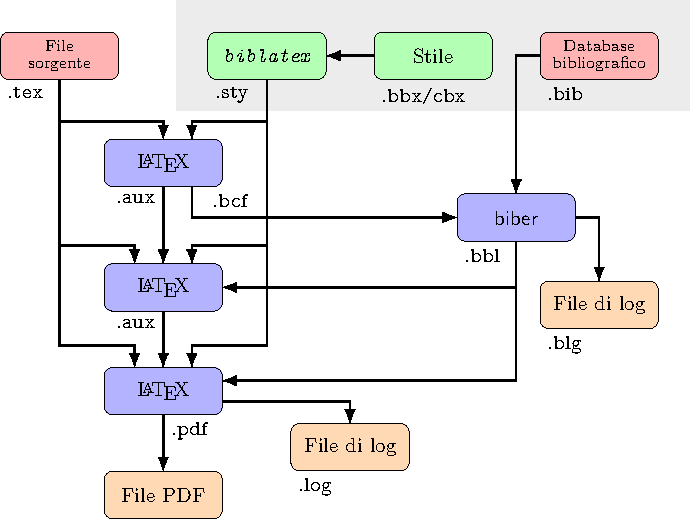
\includegraphics[width=\linewidth]{passages}
\put(-1.5,0){\rotatebox{90}{\footnotesize Diagramma creato con \pack{tikz}}}
\end{picture}
\caption{Una compilazione a 4 passaggi rappresentata graficamente.}
\medskip
\small
\begin{compactdescription}
\item[\colorbox{red!20}{rosa}]Sono i file di origine (\file{*.tex} e \file{*.bib}) e quelli finali (PDF e i file di log)
\item[\colorbox{green!20}{verde}]I file del pacchetto di stile
\item[\colorbox{blue!20}{blu}]I due programmi utilizzati nella compilazione
\item[\colorbox{black!15}{area grigia}]Indica i file che servono alla compilazione della bibliografia
\end{compactdescription}
\label{fig:1}
\end{figure}

In alcuni casi, il file di log del quarto passaggio può riportare uno dei seguenti messaggi (o entrambi):
\begin{lstlisting}[%
	style=es,
	language=TeX%
	]
LaTeX Warning:
Label(s) may have changed. Rerun to get cross-references right
\end{lstlisting}
oppure
\begin{lstlisting}[%
	style=es,
	language=TeX%
	]
Package biblatex Warning:
Please rerun LaTeX. Page breaks have changed.
\end{lstlisting}
In questo caso è necessario effettuare un quinto passaggio, sempre con \LaTeX, per correggere i riferimenti interni perché durante il processo è cambiata la paginazione.



\section{Bibliografia commentata}\label{bibnote}
Tutti i principali software  prevedono un campo ``note'' dove inserire i commenti ai riferimenti bibliografici, e, quando si effettua l'esportazione su file \file{*.bib}, è possibile esportare anche tale campo. In Bib\LaTeX\ il campo si chiama \texttt{annotation}, retro--compatibile con il campo \texttt{annote} di \hologo{BibTeX}.%
\footnote{In Bib\LaTeX\ il campo \texttt{annote} è lo \eng{short name} per il campo \texttt{annotation} per cui si possono utilizzare indifferentemente.}
Per far comparire in bibliografia i commenti, a seconda dello stile utilizzato può essere sufficiente inserire l'opzione corrispondente al momento di caricare il pacchetto \pack{biblatex}: per lo stile \pack{windycity} utilizzato in questa guida è \verb!annotate=true!. Si faccia sempre riferimento alla documentazione dello stile, consultabile con il comando \texttt{texdoc} \meta{nome pacchetto} da prompt dei comandi, per sapere se è implementata la stampa del campo \texttt{annotation} e come impostarla. Se invece lo stile scelto non prevede la stampa di tale campo, si può usare la soluzione proposta da Daniel Fowler \parencite{mendeley}, inserendo le seguenti istruzioni nel preambolo:
\begin{lstlisting}[%
	style=es,
	%language=TeX%
	]
% Use BibLaTeX for referencing
\usepackage{biblatex}
% Print annote field
\DeclareFieldFormat{annotation}{\par\textit{#1}}
\renewbibmacro*{finentry}{%
  \setunit{\finentrypunct}%
  \printfield{annotation}%
  \finentry
}
\end{lstlisting}
Se l'operazione va a buon fine, si otterrà un risultato simile alla bibliografia \LaTeX\ a pagina~\pageref{bib}.

Si faccia attenzione a non confondere il campo \texttt{annotation} con il campo \texttt{note}, previsto sia da \hologo{BibTeX} che da Bib\LaTeX. Il primo serve, come abbiamo visto, a inserire dei commenti ai riferimenti bibliografici che saranno visibili in bibliografia; il secondo invece è un campo a disposizione per inserire delle informazioni bibliografiche che non possono essere inserite in altri campi, un caso tipico è quello delle ristampe anastatiche. A scopo esemplificativo, si veda la voce \emph{I promessi sposi} \parencite{sposi}, inserita nella lista di opere consultate a pagina~\pageref{bib2}.

\backmatter
%\clearpage
\phantomsection
%\sloppy
%\emergencystretch 3em
%\begin{refsection}[guida.bib]
\label{bib}
\printbibliography[title={Bibliografia \LaTeX},keyword=latex]
\nocite{*}
%\end{refsection}
\clearpage
\printbibliography[title={Altre opere citate},keyword=others]
\label{bib2}
\end{document}
